%%%%%%%%%%%%%%%%%%%%%%%%%%%%%%%%%%%%%%%%%%%%%%%%%%%%%%%%%%%%%%%%%%%%%%%%
% Preamble
%%%%%%%%%%%%%%%%%%%%%%%%%%%%%%%%%%%%%%%%%%%%%%%%%%%%%%%%%%%%%%%%%%%%%%%%
\documentclass[11pt]{article}
%
% Packages and other includes
% Pagination
\usepackage[letterpaper, margin=1in]{geometry}
\usepackage{emptypage}
\usepackage{ulem}
\usepackage{xcolor}
\usepackage{mhchem}
%
% Fonts
\usepackage[T1]{fontenc} % best for Western European languages
\usepackage{lmodern} % Latin Modern instead of CM
\usepackage{textcomp} % required to get special symbols
%
% Math
\usepackage{amsmath, amssymb}
\usepackage{braket}
%
% Graphics, floats, tables
\usepackage{graphicx, color, float, array}
%
% Hyperlinks
\usepackage{hyperref}
%
%
% Definitions and settings
% Paragraph indent and spacing
\setlength{\parskip}{0.4\baselineskip}
\setlength{\parindent}{0in}
%
%
% Title, authors, date
\title{\textbf{Worksheet 8}}
\date{\vspace{-2em}March 4th, 2022}
%
%
%%%%%%%%%%%%%%%%%%%%%%%%%%%%%%%%%%%%%%%%%%%%%%%%%%%%%%%%%%%%%%%%%%%%%%%%
% Main document
%%%%%%%%%%%%%%%%%%%%%%%%%%%%%%%%%%%%%%%%%%%%%%%%%%%%%%%%%%%%%%%%%%%%%%%%
%

\begin{document}

\maketitle

Collaborations are encouraged and students must report all collaborators
on each assignment. All external sources (websites, books) must be
cited. An \textit{extra credit} (\textit{EC}) problem will be available per
assignment. Please submit a completed homework on-time to receive \textit{EC}
and no partial \textit{EC} (all parts must be correct) will be given out.
Additional problems are listed at the end of each assignment. This week's
assignment is due \textit{Tuesday, March 8th at 2:00pm.}

1. \textbf{Phase Diagram} The phase diagram for carbon is shown in Fig. \ref{fig:carb}.
Answer the following questions:

(a) At 3000K, what is the minimum pressure needed before graphite changes into
diamond?

(b) What is the minimum temperature at which liquid carbon exist at pressures
below 10,000 atm?

(c) Based on the phase diagram, are diamonds stable under normal conditions e.g.
1 atm and room temperature? If not, why are people able to wear diamonds without
keeping them under high pressure?

\begin{figure}[hbpt]
  \centering
  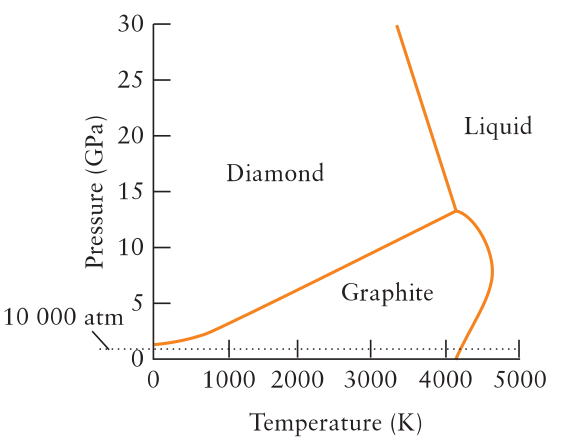
\includegraphics[scale=0.4]{carbon.png}
  \caption{Phase diagram for carbon}
  \label{fig:carb}
\end{figure}

\pagebreak

2. \textbf{Vapor Pressure}

3. \textbf{Clausius--Clapeyron Equation} The Clausius--Clapeyron equation
relates the vapor pressure and temperature of the system given by
\begin{equation}
  P_f = P_i e^{-\frac{\Delta H^\circ_\text{vap}}{R}(\frac{1}{T_2}-\frac{1}{T_1})}
\end{equation}
where $P$ is the vapor pressure, $T$ is the temperature, and $\Delta H^\circ_\text{vap}$
is the enthalpy of vaporization.

(a) At ground level, the vapor pressure of water at 80$^\circ$C is 355.26 Torr.
Determine the $\Delta H^\circ_\text{vap}$ for water. \textit{Hint: What is the
  vapor pressure of water at $100^\circ$C?}

(b) Using the $\Delta H^\circ_\text{vap}$ in part (a), determine the amount of energy
needed to heat 1 L of water from $10^\circ$C to $120^\circ$C? Heat capcities of liquid
water and water vapor are 4.184 J/(g $^\circ$C) and 1.996 J/(g $^\circ$C), respectively.

\vspace{3in}

4. 

\vfill
\textbf{Optional Additional Problems:} Ch. 11 - odd problems $35 - 45$,
$53 - 89$

Ch. 13 - odd problems $65 - 93$

Ch. 12 - odd problems $27 - 51$, $77 - 89$

\end{document}
